\documentclass[12pt]{report}
\usepackage{graphicx}
\usepackage{subfig}
\usepackage{listings}
\usepackage{hyperref}

\begin{document}
\lstset{language=Python}

\title{Homework 2: Applied Machine Learning}
\author{Tim Delisle and Sam Raudabaugh}
\date{09/29/2015}
\maketitle

\noindent{{\large 1. Face Recognition}}

For this assignment, we investigated a subset of the Yale Face Database. Our goal was to
train a logistic regression classifier that uses eigenfaces to predict which subject is
portrayed in the image.

Once again, we use the \verb+LogisticRegression+ model contained in \verb+scikit-learn+
for this classification. To train the classifier, however, we must first obtain the mean face
$\mu$ from computing the average grayscale intensity of each pixel across the training set.
The mean face is shown in Figure 1.

\begin{figure}
\centering
  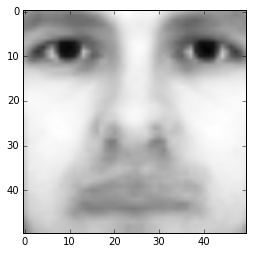
\includegraphics[width=75mm]{figures/mean.png}
\caption{Mean face image}
\end{figure}

We then subtract this from every image and perform Singular Value Decomposition (SVD) on the
dataset to compute the eigenfaces, an example of which is shown in Figure 2. Using the SVD
factors $U$, $\Sigma$, and $V^T$, where $V^T$ is the matrix of eigenfaces, we can construct
low-rank approximations by truncating the number of elements in each factor.

\begin{figure}
\centering
  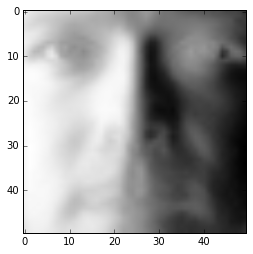
\includegraphics[width=75mm]{figures/eigen.png}
\caption{Example eigenface}
\end{figure}

In Figure 3, a plot of approximation error versus $r$, the number of eigenfaces (first $r$
rows of $V^T$) used in the approximation, is presented. To better understand how our classifier
will perform, we examine the relationship between information loss and the size of the subset of
eigenfaces, and see that the error slope is fairly asymptotic for $r > 100$.

\begin{figure}
\centering
  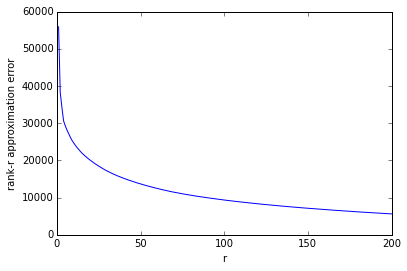
\includegraphics[width=75mm]{figures/error.png}
\caption{Plot of approximation error}
\end{figure}

To use a logistic regression classifier with this data, we build feature matrices out of the
training and test images by projecting them on the subset of eigenfaces (i.e.\ multiplying
$XV^T[:r,:]$). At $r = 10$, the logit model performs with classification accuracy 0.61. Based
on the previous plot of approximation error in Figure 3, we would expect our classifier
to see little improvement in accuracy beyond $r = 100$, and in fact, the plotted accuracy
in Figure 4 shows that this is the case.

\begin{figure}
\centering
  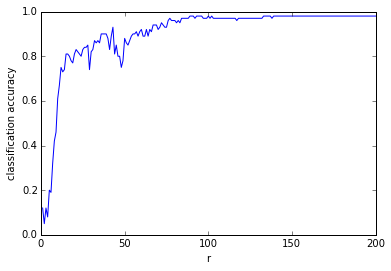
\includegraphics[width=75mm]{figures/accuracy.png}
\caption{Plot of classifier accuracy}
\end{figure}

\end{document}
